\subsection{Integration Lemmas}
During the course of this thesis we will see some recurring patterns in the
integrals that need to be solved. We will thus list some explicit formulas for
them now and prove the simpler ones here.

The first one is a classical result of asymptotic analysis and is the basis of
most further results on the asymptotics of exponential integrals.
\begin{Lemma}[Watson]
  Let $\phi\colon [0,1] \to \mathbb{C}, \phi(t) = t^\sigma g(t)$ such that $g$ is
analytic in some neighbourhood of $t=0$, $\sigma > -1$, $\beta > 0$, and
\begin{equation*}
  \exists C, b > 0\, \forall t > 0\colon \Abs{\phi(t)} < C \Eto{bt}.
\end{equation*}
Then the exponential integral
\begin{align*}
  F(x) := \Integ[T]{0}{t}{\Eto{-\beta\,xt}\phi(t)}.
\end{align*}
is finite for all $x \geq 0$ and has the asymptotic expansion in terms of the
gamma function $\Gamma$ (cf.\ \cref{app:gamma})
\begin{equation*}
  F(x)\SimAs{x\to\infty}\sum_{n=0}^{\infty}
  \frac{g^{(n)}(0)}{(\beta x)^{n+\sigma+1}} \frac{\Gamma(n+\sigma+1)}{n!}
\end{equation*}

  \begin{proof}
    Since the proof is a bit lengthy and not needed to understand the following
    it can be found in Appendix~\ref{sec:proof-watson}.
  \end{proof}
%    \begin{Remark}
%        We actually don't need analyticity but only the existence of as many
%        derivatives as degrees we want and additionally a finiteness condition
%        on .
%    \end{Remark}
\end{Lemma}

The next lemma considers the continuity properties of exponential integrals like
the ones that are object of Watson's Lemma:
\begin{Lemma}
  \label{lem:continuity_of_watson_integrals}
  Let $f\colon [0,T)\to\mathbb{R}$ (where $T$ may be $\infty$) be an integrable
  function. Then the exponential parameter integral
  \begin{align*}
    F(x) = \Integ[T]{0}{t}{\Eto{-tx} f(t)}
  \end{align*}
  is continuous in $x$.
  \begin{Proof}
    The statement follows immediately from a classical result of Lebesgue theory
    on the continuity of parameter-dependent integrals (REF: Königsberger 2
    282f). We only need to check, that there is an integrable majorant for all
    $x$, which is simply $f(t)$ in this case, and that the whole integrand is
    continuous in $x$ for fixed $t$ which is obvious.
  \end{Proof}
\end{Lemma}

The third lemma is a quite general formula for nested integrals, in which the
upper limit of the inner integral is the integration variable of the outer one:
\begin{Lemma}
    \label{lem:triangle-integration}
    Let $f,g\colon[0,1]\to\mathbb{R}$ be continuous. Then the following formula
    holds:
    \begin{align*}
        \Integ[1]{0}{x}{g(x)\Integ[1]{x}{y}{f(y)}} =
        \Integ[1]{0}{y}{f(y)\Integ[y]{0}{x}{g(x)}}
    \end{align*}
    \begin{proof}
        Let $F(x) := \Integ[x]{0}{y}{f(y)}$ and $G(y) := \Integ[y]{0}{x}{g(x)}$.
        Then we see using partial integration:
        \begin{align*}
            \Integ[1]{0}{x}{g(x)\Integ[1]{x}{y}{f(y)}} &=
            \Integ[1]{0}{x}{g(x)F(1)} - \Integ[1]{0}{x}{g(x)F(x)} \\
            &= G(1)F(1) - \left(\Bigl.G(y)F(y)\Bigr|_0^1 -
            \Integ[1]{0}{y}{G(y)f(y)}\right) \\
            &= \Integ[1]{0}{y}{G(y)f(y)} =
            \Integ[1]{0}{y}{f(y)\Integ[y]{0}{x}{g(x)}},
        \end{align*}
        which proves the given formula.
    \end{proof}
\end{Lemma}

\begin{Remark}
  This is in fact only Fubini's theorem for the integral of $(x,y)\to g(x)f(y)$
  over a right-angled triangle:
  \begin{center}
    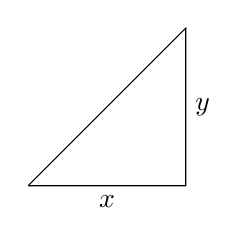
\begin{tikzpicture}
      \draw (0,0)
      -- (2,2)
      -- node[anchor=west] {$y$} (2,0)
      -- node[anchor=north] {$x$} (0,0);
    \end{tikzpicture}
  \end{center}
\end{Remark}

Finally we give a formula for a particular kind of integral that comes up a lot
in the final calculations:
\begin{Lemma}
  \label{lem:beta_function_formula}
  Let $a, b > 0$ and $m > n$. Then
  \begin{align*}
    \Integ[\infty]{0}{x}{\frac{x^n}{(a^2 + b^2 x^2)^{m}}} =
    \frac{a^{n-2m+1}}{2b^{n+1}}B\bigl(\tfrac{n+1}{2}, \tfrac{2m - n -
    1}{2}\bigr),
  \end{align*}
  where $B$ denotes the Beta function.
  \begin{Proof}
    \begin{align*}
      \Integ[\infty]{0}{x}{\frac{x^n}{(a^2 + b^2 x^2)^{m}}} 
      &= \frac{a^{n-2m+1}}{b^{n+1}} \Integ[\infty]{0}{y}{\frac{y^n}{(1 +
  y^2)^m}}
        &\text{with $y = bx / a$} \\
        &= \frac{a^{n - 2m + 1}}{2b^{n+1}}
        \Integ[\infty]{0}{z}{\frac{z^{\frac{n-1}{2}}}{(1 + z)^n}}
        &\text{with $z = \sqrt{y}$}\\
        &= \frac{a^{n-2m+1}}{2b^{n+1}}B\bigl(\tfrac{n+1}{2}, \tfrac{2m - n -
      1}{2}\bigr)
    \end{align*}
    The formula used in the last step is proven in the Appendix
    \ref{sec:beta_function}.
  \end{Proof}
\end{Lemma}
